% Short class version (at most 3 pages) of brexit-game.tex: tasks (i)-(vii) of intrucoes.md.
% Compile: pdflatex brexit-game-short.tex (twice). Check: pdffonts (all Type 1, uni = yes).
% Every number is copied from brexit-game.tex, which brexit-check.py asserts; none is new here.
\documentclass[10pt,a4paper]{article}
\usepackage[utf8]{inputenc}
\usepackage[T1]{fontenc}
\usepackage{lmodern}   % Type 1 vector fonts (replaces PK bitmaps)
\usepackage{cmap}      % ToUnicode CMap -> copyable text and accents
\usepackage[english]{babel}
\usepackage{amsmath,amssymb,mathtools}
\usepackage[a4paper,margin=1.8cm,top=1.6cm,bottom=1.6cm]{geometry}
\usepackage{microtype}
\usepackage{booktabs,array}
\usepackage{enumitem}
\usepackage{xcolor}
\usepackage{tikz}
\usepackage[most]{tcolorbox}
\usepackage{fancyhdr}
\usepackage[hidelinks]{hyperref}

\setlist{topsep=2pt,itemsep=1pt}
\setlength{\parindent}{0pt}
\setlength{\parskip}{4pt}

\pagestyle{fancy}\fancyhf{}
\lhead{\footnotesize Economics of Organizations and Incentives --- MPE Insper}
\rhead{\footnotesize Case: the Brexit negotiation as a game (short version)}
\cfoot{\footnotesize\thepage}
\renewcommand{\headrulewidth}{0.3pt}
\setlength{\headheight}{13pt}

\makeatletter
\renewcommand\section{\@startsection{section}{1}{\z@}{6pt plus 2pt}{2pt}{\normalfont\large\bfseries}}
\makeatother

\definecolor{ans}{RGB}{20,110,70}
\definecolor{src}{RGB}{30,80,150}
\newcommand{\gbp}{\pounds}
\newcommand{\Nt}{\mathit{Nt}}
\newcommand{\dF}{\mathit{F}}
\newcommand{\dU}{\mathit{U}}

% One UK decision node with its Present/Reject edges, the vote and three leaves (as in brexit-game.tex).
% #1 index of its top leaf, #2 parent EU node, #3 deal label, #4-#6 payoffs (pass, fail, reject),
% #7 style of the EU edge, #8 style of the present edge, #9 style of the reject edge.
\newcommand{\branch}[9]{%
  \node[dec,label={[font=\tiny,inner sep=1pt]above:UK}] (u#1) at (4,{#1+1}) {};
  \node[nat,label={[font=\tiny,inner sep=1pt]above:Parl.}] (n#1) at (6,{#1+0.5}) {};
  \draw[#7] (#2) -- node[lab]{#3} (u#1);
  \draw[#8] (u#1) -- node[lab,above,sloped]{present} (n#1);
  \draw[#9] (u#1) -- node[lab,below,sloped,pos=0.4]{reject} (8,{#1+2});
  \draw[e] (n#1) -- node[lab,above,pos=0.6]{$0.8$} (8,#1);
  \draw[e] (n#1) -- node[lab,below,pos=0.6]{$0.2$} (8,{#1+1});
  \node[right] at (8,#1) {#4};
  \node[right] at (8,{#1+1}) {#5};
  \node[right] at (8,{#1+2}) {#6};
}

\begin{document}

\begin{center}
{\Large\bfseries Boris's Brexit Dilemma as a Game --- class version}\\[2pt]
{\small Lecture 3 case. Short version of \texttt{Cases/Brexit/brexit-game.pdf}, where every step,
variant and reference is worked out. Costs in \gbp bn; payoff $=-$cost; players are risk neutral.}
\end{center}

\section*{(i) Players}
\begin{itemize}[leftmargin=1.4em]
  \item \textbf{UK} (Boris Johnson's government): prepares or not; presents the EU's offer to Parliament or rejects it.
  \item \textbf{EU} (chief negotiator Michel Barnier): chooses which deal to offer.
  \item \textbf{Parliament, modelled as Nature}: passes a presented deal with probability $p=0.8$, fails it with $0.2$.
\end{itemize}

\section*{(ii) Timing and actions}
\begin{enumerate}[label=\textbf{Stage \arabic*.},leftmargin=4.6em]
  \item \textbf{UK}: \emph{Prepare} ($P$) or \emph{Not prepare} ($N$). Preparation costs $\kappa=5$, is all-or-nothing and sunk; it saves $m=12.5$ of the hard-Brexit cost.
  \item \textbf{EU}: offers a deal $d\in\{\dF,\Nt,\dU\}$ (favourable, neutral, unfavourable to the UK).
  \item \textbf{UK}: \emph{presents} the deal to Parliament or \emph{rejects} it (hard Brexit, plus a political cost $r\ge0$; baseline $r=0$).
  \item \textbf{Nature}: the deal passes ($0.8$) or fails ($0.2$, hard Brexit, no $r$).
\end{enumerate}
Strategies: $\lvert S_{UK}\rvert=2\times2^6=128$, $\lvert S_{EU}\rvert=3^2=9$.

\section*{(iii) Information}
\textbf{Baseline: the EU observes preparation} (stockpiles and border infrastructure are visible); the
UK sees the offer before deciding. Every information set is a singleton; the only uncertainty is
the vote, whose probability is common knowledge. \textbf{Variant:} if the EU does not observe
preparation, its two nodes form one information set, so stages 1 and 2 are effectively simultaneous
(solved in the box below).

\section*{(iv) Payoffs}
Inputs (costs): hard Brexit UK 35, EU 18; deals $(c_d,e_d)$: $\dF$ $(19,13)$, $\Nt$ $(23,9)$,
$\dU$ $(27,5)$. A prepared UK's hard-Brexit cost is $35-12.5+5=27.5$; in a soft Brexit it pays $c_d+5$.
The 18 leaves carry 8 distinct payoff pairs (UK, EU):

\begin{center}\small
\begin{tabular}{llccc}
\toprule
UK prepared? & Event & $\dF$ & $\Nt$ & $\dU$ \\
\midrule
$N$ & deal passes   & $(-19,-13)$ & $(-23,-9)$ & $(-27,-5)$ \\
$N$ & vote fails    & $(-35,-18)$ & $(-35,-18)$ & $(-35,-18)$ \\
$N$ & UK rejects    & $(-35-r,-18)$ & $(-35-r,-18)$ & $(-35-r,-18)$ \\
\midrule
$P$ & deal passes   & $(-24,-13)$ & $(-28,-9)$ & $(-32,-5)$ \\
$P$ & vote fails    & $(-27.5,-18)$ & $(-27.5,-18)$ & $(-27.5,-18)$ \\
$P$ & UK rejects    & $(-27.5-r,-18)$ & $(-27.5-r,-18)$ & $(-27.5-r,-18)$ \\
\bottomrule
\end{tabular}
\end{center}
\textbf{Why this ordering:} an unprepared UK prefers every deal to no deal ($27<35$); a prepared UK,
net of the sunk 5, prefers no deal to $\Nt$ and $\dU$ but not to $\dF$ ($19<22.5<23<27$); the EU
prefers less generous deals and any deal to no deal ($5<9<13<18$), and is hurt less by no deal than the UK ($18<35$).

\section*{(v) The game tree}
\begin{center}
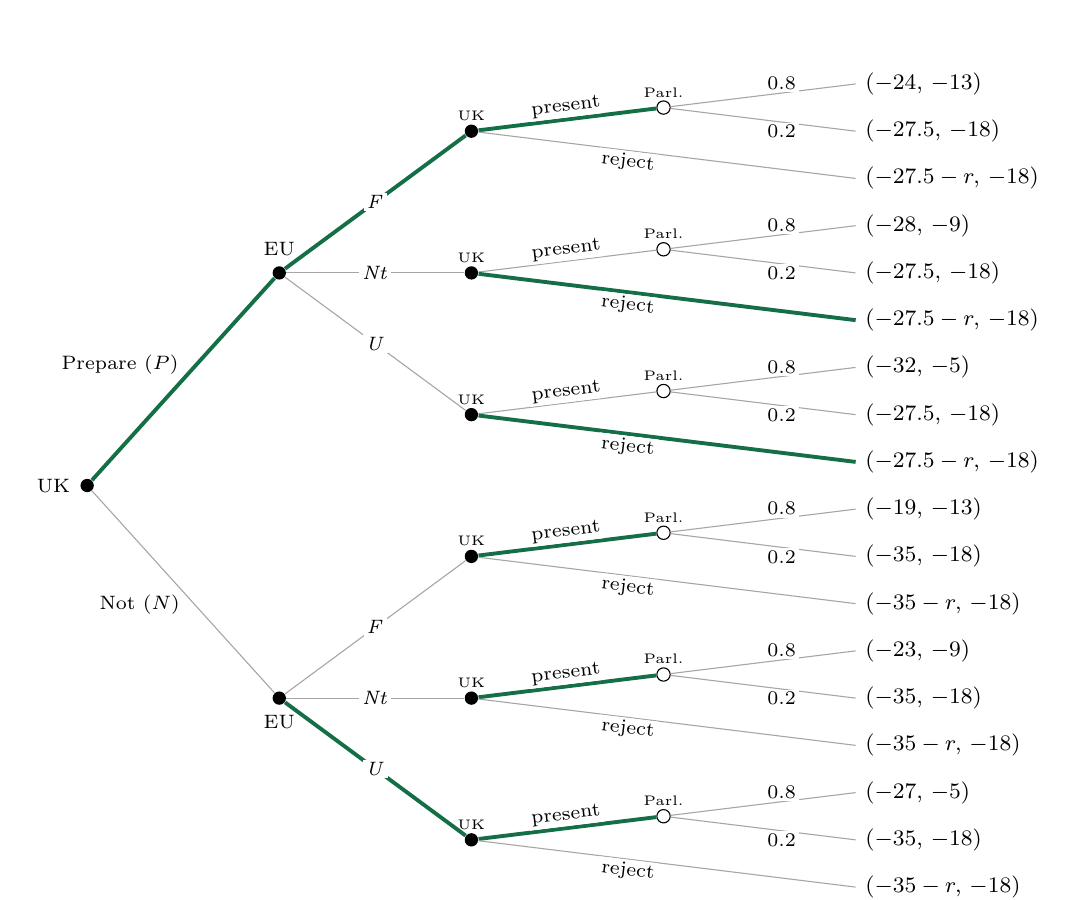
\begin{tikzpicture}[x=1.22cm,y=-0.60cm,every node/.style={font=\footnotesize},
  dec/.style={circle,fill=black,inner sep=1.7pt},
  nat/.style={circle,draw,fill=white,inner sep=1.7pt},
  e/.style={draw=gray!70,thin},
  spe/.style={draw=ans,line width=1.4pt},
  lab/.style={font=\scriptsize,fill=white,inner sep=1pt}]
  \node[dec,label={[font=\scriptsize]left:UK}] (r) at (0,8.5) {};
  \node[dec,label={[font=\scriptsize]above:EU}] (eP) at (2,4) {};
  \node[dec,label={[font=\scriptsize]below:EU}] (eN) at (2,13) {};
  \draw[spe] (r) -- node[lab,above left]{Prepare ($P$)} (eP);
  \draw[e] (r) -- node[lab,below left]{Not ($N$)} (eN);
  \branch{0}{eP}{$\dF$}{$(-24,\,-13)$}{$(-27.5,\,-18)$}{$(-27.5-r,\,-18)$}{spe}{spe}{e}
  \branch{3}{eP}{$\Nt$}{$(-28,\,-9)$}{$(-27.5,\,-18)$}{$(-27.5-r,\,-18)$}{e}{e}{spe}
  \branch{6}{eP}{$\dU$}{$(-32,\,-5)$}{$(-27.5,\,-18)$}{$(-27.5-r,\,-18)$}{e}{e}{spe}
  \branch{9}{eN}{$\dF$}{$(-19,\,-13)$}{$(-35,\,-18)$}{$(-35-r,\,-18)$}{e}{spe}{e}
  \branch{12}{eN}{$\Nt$}{$(-23,\,-9)$}{$(-35,\,-18)$}{$(-35-r,\,-18)$}{e}{spe}{e}
  \branch{15}{eN}{$\dU$}{$(-27,\,-5)$}{$(-35,\,-18)$}{$(-35-r,\,-18)$}{spe}{spe}{e}
\end{tikzpicture}

{\footnotesize Filled dots: decision nodes; open dots: Parliament (upper edge pass, $0.8$; lower
edge fail, $0.2$). Thick green: the SPE action at every node, on and off the path, for $r<0.4$ and $k\le5$.}
\end{center}

\section*{(vi) Backward induction and the SPE}
\textbf{Step 1 (UK: present or reject).} After $N$, presenting $d$ costs $0.8\,c_d+0.2\times35$:
$\dF$ 22.2, $\Nt$ 25.4, $\dU$ 28.6, all below $35+r$, so \emph{present every deal}. After $P$,
presenting costs $0.8\,(c_d+5)+0.2\times27.5$: $\dF$ 24.7, $\Nt$ 27.9, $\dU$ 31.1, against 27.5 for
rejecting, so \emph{present $\dF$, reject $\Nt$ and $\dU$}.

\textbf{Step 2 (EU: offer).} A presented deal costs the EU $0.8\,e_d+3.6$: $\dF$ 14, $\Nt$ 10.8,
$\dU$ 7.6; a rejection costs 18. After $N$ everything is presented: offer $\dU$ (7.6). After $P$
only $\dF$ is presented: offer $\dF$ (14 beats 18).

\textbf{Step 3 (UK: prepare?).} $P$ leads to $(-24.7,-14)$, $N$ to $(-28.6,-7.6)$. Since $24.7<28.6$, the UK \emph{prepares}.

\begin{tcolorbox}[colback=ans!5,colframe=ans,boxrule=0.6pt,left=5pt,right=5pt,top=3pt,bottom=3pt]
\textbf{SPE} (baseline, $r=0$, $k=0$):
\begin{align*}
  s^*_{UK} &= \bigl(P;\ \text{after }P\text{: present }\dF,\ \text{reject }\Nt,\ \text{reject }\dU;\
              \text{after }N\text{: present }\dF,\Nt,\dU\bigr),\\
  s^*_{EU} &= \bigl(\dF\text{ after }P;\ \dU\text{ after }N\bigr),
\end{align*}
with Parliament passing a presented deal with probability 0.8. Path: $P$, $\dF$, present; payoffs
$(-24,-13)$ with probability 0.8, $(-27.5,-18)$ with probability 0.2. \textbf{Expected payoffs
$(-24.7,\,-14)$}, against $(-28.6,\,-7.6)$ without preparation. The UK gains 3.9, the EU loses 6.4;
the 2.5 difference is a deadweight loss.
\end{tcolorbox}

\begin{tcolorbox}[colback=src!4,colframe=src,boxrule=0.5pt,left=5pt,right=5pt,top=3pt,bottom=3pt,
  title={Key comparative statics}]
\begin{itemize}[leftmargin=1.2em]
  \item \textbf{Political cost of walking away, $r$} (a prepared UK presents $d$ iff $c_d\le22.5+r/0.8$):
    $r<0.4$: $(P,\dF)$, UK $-24.7$, EU $-14$;\quad
    $0.4<r<3.6$: $(P,\Nt)$, UK $-27.9$, EU $-10.8$;\quad
    $r>3.6$: $(N,\dU)$, UK $-28.6$, EU $-7.6$.
    A higher $r$ makes the threat costlier to carry out, so it \emph{weakens} it.
  \item \textbf{EU deterrence premium $k$} on an implemented $\dF$ (cost $13+k$): after $P$ the EU
    offers $\dF$ iff $0.8\,(13+k)+0.2\times18\le18$, i.e.\ $k\le5$. For $k>5$ the prepared UK
    rejects and the outcome is a hard Brexit, $(-27.5,\,-18)$.
  \item \textbf{Unobservable preparation}: no pure equilibrium (best responses cycle). Mixed
    equilibrium $\sigma=\Pr(P)=8/13$, $\tau=\Pr(\dF)=11/36$; UK $-1199/45\approx-26.64$ (versus
    $-24.7$ when observed), EU $-14$; talks break down with probability $50/117\approx0.43$.
    Hidden commitment is no commitment.
\end{itemize}
\end{tcolorbox}

\clearpage
\begin{tcolorbox}[colback=src!4,colframe=src,boxrule=0.5pt,left=4pt,right=4pt,top=3pt,bottom=3pt,
  title={In-class decision guide (baseline numbers)}]
\small
\begin{minipage}[t]{0.485\linewidth}
\textbf{Playing the UK}
\begin{itemize}[leftmargin=1.1em]
  \item \textbf{Prepare, and make sure the EU sees it.} Visible preparation is worth 3.9 at
    $p=0.8$ (and $3p+7.5(1-p)>0$ for any $p$); hidden preparation is worth far less.
  \item \textbf{If prepared}, present $d$ iff $c_d\le22.5+r/p$: present only $\dF$ while $r<0.4$;
    if $0.4<r<3.6$, present $\dF$ or $\Nt$ and reject $\dU$; if $r>3.6$, do not prepare at all.
  \item \textbf{If unprepared, present whatever is offered} ($c_d\le35+r/p$ always holds): every
    deal beats no deal, and saying otherwise is cheap talk.
  \item \textbf{If the EU's deterrence concern is large} ($k>5$), expect a breakdown; you still
    prefer to have prepared ($27.5<28.6$).
\end{itemize}
\end{minipage}\hfill
\begin{minipage}[t]{0.485\linewidth}
\textbf{Playing the EU}
\begin{itemize}[leftmargin=1.1em]
  \item \textbf{If you see preparation, offer $\dF$}, unless you believe the UK's $r$ is high.
    If unsure, offer $\Nt$ instead of $\dF$ only if $\Pr(r\ge0.4)>5/9$, and $\dU$ instead of $\dF$
    only if $\Pr(r\ge3.6)>5/13$ (from $q\times10.8+(1-q)\times18=14$ and $q\times7.6+(1-q)\times18=14$).
  \item \textbf{If you see no preparation, offer $\dU$.} It will be presented.
  \item \textbf{If you cannot tell}, the equilibrium has you offering $\dF$ with probability
    $11/36$ and $\dU$ otherwise; in practice, invest in finding out.
  \item \textbf{Weigh precedent.} If rewarding a leaver costs you more than 5 in deterrence,
    refuse $\dF$ and accept that a hard Brexit follows.
\end{itemize}
\end{minipage}
\end{tcolorbox}

\section*{(vii) Why your negotiation may differ from the SPE}
\begin{itemize}[leftmargin=1.4em]
  \item \textbf{Cheap talk versus commitment.} ``No deal is better than a bad deal'' changes nothing
    unless backed by preparation; an EU that believes an unprepared UK's threat plays a Nash
    equilibrium that is not subgame perfect, with payoffs $(-22.2,\,-14)$.
  \item \textbf{Fairness.} Lab responders reject splits they find insulting; the surplus here is
    $53-32=21$, and $\dF$, $\Nt$, $\dU$ give the UK about 76\%, 57\%, 38\% of it. An EU player may
    refuse $\dF$ as unfair to the EU.
  \item \textbf{Reputation and repeated interaction.} The EU faces 27 members and future
    applicants (the premium $k$), and both sides negotiate again later.
  \item \textbf{Uncertainty and deadlines.} Private information about $r$ or $p$ can make rational
    bargaining break down; a rejection that leads to an extension turns the game into alternating
    offers, where patience matters.
\end{itemize}
Record your pair's moves against the SPE in the template at the end of \S11 of
\texttt{brexit-game.pdf} (``Template: record your negotiation against the SPE'').

\end{document}
